\documentclass[conference,10pt]{IEEEtran}
\usepackage{fancyhdr}
\usepackage{amssymb}
\usepackage{amsmath}
\usepackage{amsfonts}
\usepackage[T1]{fontenc} % get tt fonts to work right
\usepackage{graphicx}
\usepackage{multirow}
\usepackage{color}
\usepackage{caption}
\DeclareCaptionType{copyrightbox} % workaround for bug in caption
\usepackage{subcaption}
\usepackage{xspace}
\usepackage{url}

\begin{document}

\special{papersize=8.5in,11in}
\setlength{\pdfpageheight}{\paperheight}
\setlength{\pdfpagewidth}{\paperwidth}


\title{Mapping HALO Exchange onto Toruses and Stuff}

\author{\IEEEauthorblockN{
Timothy G. Armstrong,\IEEEauthorrefmark{1}
Yadu Nand\IEEEauthorrefmark{1}\IEEEauthorrefmark{2}\IEEEauthorrefmark{3}}
  \IEEEauthorblockA{
  \IEEEauthorrefmark{1}Dept. of Computer Science,
    University of Chicago,
    Chicago, IL, USA}
  \IEEEauthorblockA{\IEEEauthorrefmark{2}Mathematics and Computer Science Division,
    Argonne National Laboratory,
    Argonne, IL, USA}
  \IEEEauthorblockA{\IEEEauthorrefmark{3}Computation Institute,
    University of Chicago and Argonne National Laboratory,
    Chicago, IL, USA}
}

\maketitle

 
\begin{abstract}
Abstract goes here
\end{abstract}

\section{Introduction}
We're going to cite Swift/T~\cite{SwiftT_2013} and include an illustration
(see Figure~\ref{fig:task-data}). 

\begin{itemize}
  \item A bullet point
\end{itemize}

\subsection{Abstract Execution Model}
\label{sect:ddt-model}
\begin{figure}
  \center
  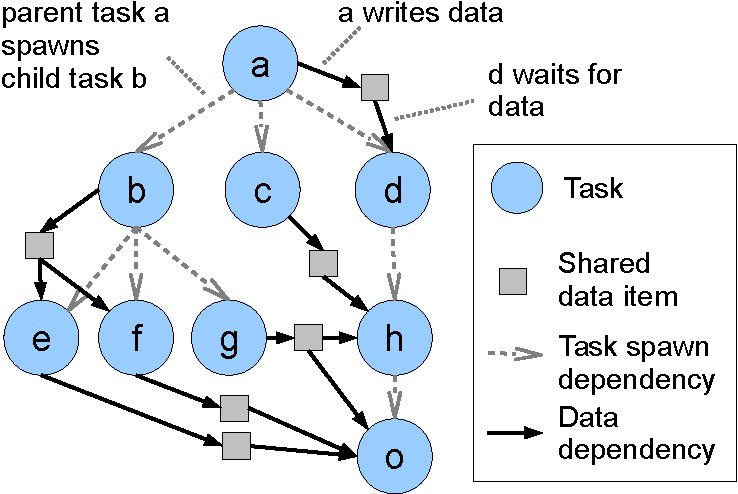
\includegraphics[width=0.325\textwidth]{fig/task-data}
  \caption{This is a figure.
    \label{fig:task-data}}
\end{figure}

\bibliographystyle{abbrv}
\bibliography{halo}

\end{document}
